\documentclass[a4paper,12pt,final,oneside,openright]{article}
\usepackage{report}
\usepackage{amsmath,amssymb}
\usepackage{graphicx}

\newcommand{\reporttitle}{Machine Learning - Advanced Course}
\newcommand{\enseignants}{
Carl Henrik~\textsc{Ek}\\
Hedvig~\textsc{Kjellström}\\
Jens~\textsc{Lagergren}}

\newcommand{\reportauthor}{
Thayabaran~\textsc{Kathiresan}\\
Rémi~\textsc{Domingues}\\
Agnes Martine~\textsc{Nielsen}\\
Tobias~\textsc{Wiens}}
% \newcommand{\hexanome}{H4211}
\newcommand{\reportsubject}{}
\newcommand{\stagetopic}{Kernel Principal Component Analysis}
\newcommand{\dateperiod}{November $24^{th}$ - December $17^{th}$}
\newcommand{\HRule}{\rule{\linewidth}{0.5mm}}
\setlength{\parskip}{1ex} % Espace entre les paragraphes

\hypersetup{
    pdftitle={\reporttitle},%
    pdfauthor={\reportauthor},%
    pdfsubject={\reportsubject},%
    pdfkeywords={}
}

\title{\reporttitle}
\author{\reportauthor}

\setlongtables

%\setcounter{tocdepth}{4}
\begin{document}
    \renewcommand{\chaptername}{} %\renewcommand{\thechapter}{}
    \renewcommand{\contentsname}{Contents}

    \pagestyle{empty}
    \pagenumbering{arabic}
    \input{title}
	\pagebreak
    \sloppy          % Justification moins stricte : des mots ne dépasseront pas des paragraphes

    %\frontmatter
    \thispagestyle{empty}
    \tableofcontents
    \addtocontents{toc}{\protect\thispagestyle{empty}}
    \pagebreak

    %\mainmatter
    \pagestyle{headings}
    %\renewcommand{\chaptermark}[1]{\markboth{\MakeUppercase{\chaptername\ \thechapter.\ #1}}{}}
    %\renewcommand{\sectionmark}[1]{\markright{\thesection{} #1}}

    \section*{Introduction} % Why not just remove the * and have it add to content automatically?? -Agnes
\addcontentsline{toc}{section}{Introduction}
Principal Component Analysis is a method which aims at reducing the dimensionality of a dataset into a linearly uncorrelated set of features, each maximizing the variance on the observations.

The method presented here gather PCA and kernel methods by describing an efficient way to compute principal components in a feature space of large dimensionality that is related to the input space by a non-linear mapping. An illustration of this can be seen in Figure \ref{fig:kernel_pca}. This is achieved by the use of kernel functions similar to the ones used in Support Vector Machines (SVM). This report details how to achieve this basis transformation and apply it through a feature extraction based on a digit recognition experiment.

\begin{figure}[h!]
    \centering
    \includegraphics{img/kernel_pca.jpg}
    \caption{Comparison between linear PCA and kernel PCA}
    \label{fig:kernel_pca}
\end{figure}

    \section{Theory}
The following section describes the derivation of the method written in B. Schölkopf and A. J. Smola, \textit{Kernel principal component analysis}\cite{scholkopf1997kernel}.

The Kernel Principal Component Analysis allows us to find Principal Components which are nonlinearly related to the input space. Giving the possibility to extract and find relevant data having a nonlinear relation in the input space.

%This statement is not accurate, so i have taken the introduction to 2.2 up here instead - Agnes
%The advantage of this method rely in its performances when performing PCA on high-dimensional data, even if these data have been generated using a non-linear transformation from their initial space by the use of a kernel function. Therefore, it should give better result than standard PCA (using maximizing variance or minimum squared distance criteria\footnote{TODO: check if correct}) when applied to such a dataset.

\subsection{Concepts}
\subsubsection{Kernel} \label{sec:kernel}
The kernels mentioned in this report refer to functions used to represent an inner product in a high-dimensional feature space which arise from a non-linear transformation from an input space. That means a kernel function $k$ is,

\begin{equation}
k(\textbf{x},\textbf{x'}) = (\Phi(\textbf{x})\cdot\Phi(\textbf{x'}))
\end{equation}

where $\Phi: \mathbb{R}^N\rightarrow F$ is a non-linear mapping from an input space $\mathbb{R}^N$ to a feature space $F$. $\textbf{x},\textbf{x'}\in \mathbb{R}^N$, and $(\bullet\cdot\bullet)$ denotes the inner product in $F$. 

The main interest of kernel functions resides in their computation cost, since they provide an inner product between each pair of points in the high dimension space for a lower complexity than the effective computation of the coordinates of the input points in the high dimension space followed by their pairwise inner product\cite{boser1992training}.

The efficiency of kernels when applied to Support Vector Machines has been demonstrated\cite{scholkopf1996incorporating}. In the experiments, we will work with a polynomial kernel.
\begin{align}
\text{Polynomial of degree \textit{d}: }& k(x,y) = (x \cdot y)^d
\end{align}


% I think this whole section is basic knowledge and unnescessary. -Agnes
%\subsubsection{Eigenvalues and eigenvectors\label{sec:eigen_concept}}

%The eigenvalues \textit{$\lambda$} of a square matrix \textit{A} are obtained by finding the roots of the polynom obtained with the following formula:

%\begin{equation}
%|A - \lambda I| = 0
%\end{equation}

%The eigen vectors $v \neq {0}$ are then found by resolving the following equation for each eigenvalue:

%\begin{equation} \label{eq:eigenvectors_constraint}
%A v = \lambda v \Leftrightarrow (A - \lambda I) v = 0
%\end{equation}


\subsubsection{Principal Component Analysis (PCA)}
\label{sec:pca}
The following section is based on \cite{pcaTutorial}. \newline
PCA is a tool used to reduce the dimensionality of a dataset. When dealing with many input dimensions, the relevant data might be extracted using less dimensions, therefore we find a basis of orthogonal vectors in the input space, from which we know each vectors' contribution for the representing the data.  \newline
In order to find a lower dimensional representation of the data it requires to build the covariance matrix of the given dataset. Following, we extract the principal components by calculating the $N$ eigenvectors corresponding the highest eigenvalues. The $N$ is given by the user or deduced from Maximum Likelihood Estimation (MLE)\cite{minka2000automatic}. In further detail, the eigenvectors with the highest eigenvalues are chosen, because those are the eigenvectors explain the highest amount of variance in the data. \newline

The idea behind PCA is to "diagonalize the covariance matrix", in detail: we try to map our data into a new representation denoted by:

\begin{equation} \label{eq:pca_projection}
\textbf{Y} = \textbf{PX}
\end{equation}

Where $ \textbf{X} $ is our data and $ \textbf{Y} $ is our new representation. The matrix $\textbf{P}$ is the orthonormal projection matrix, transforming \textbf{X} into the representation $ \textbf{Y} $. The target of the PCA is to transform the data into a representation $ \textbf{Y} $ in which covariance matrix is a diagonal matrix. Thereby diagonalizing the covariance matrix. When we choose $ \textbf{P} $ to be a matrix where each row is an eigenvector of $ \textbf{X} $, the covariance matrix of $ \textbf{Y} $ becomes diagonal and the matrix $ \textbf{P }$ represents our principal components, for more details see \cite{pcaTutorial}.\newline

%By reducing its dimensionality and therefore reducing the impact of curse dimensionality, the data represented in this space is then a better input for knowledge extraction methods than the one in high-dimensional space\cite{tipping1999probabilistic}.


\subsection{Kernel Principal Component Analysis}

\subsubsection{Derivation}
We define the high-dimension feature space \textit{F}, containing the image of our data obtained after a non-linear mapping $\Phi$ from the input space

\begin{equation} \label{eq:space_definition}
\Phi : \mathbb{R}^N \rightarrow F, \textbf{x} \rightarrow \textbf{X}
\end{equation}

We first assume that our data in \textit{F} is centered, $\sum\limits_{k=1}^l \Phi(\textbf{x}_k) = 0$ , i.e. the mean is 0.

As done in the standard PCA, the Kernel PCA algorithm constructs the covariance matrix of the data, but now we define it in the feature space $F$.

\begin{equation} \label{eq:cov_matrix}
\bar{C} = \frac{1}{l} \sum\limits_{j=1}^{l} \Phi(\textbf{x}_j) \Phi(\textbf{x}_j)^T
\end{equation}

% I don't understand why we have this part
%\textbf{Projecting into higher dimensional space}\newline
%Projecting the higher dimensional $\Phi(x)$ into a different space, as it was done in the normal PCA case in low dimensional space (section \ref{sec:pca}), will lead to a new representation of the input in high dimensional space. In PCA the Eigenvectors would be computed and used to get a "diagonal covariance matrix" \cite{pcaTutorial}. \newline
%In this case we cannot calculate the Eigenvectors since the $\Phi(x)$ can map into infinite dimensional space.The high dimensional eigenvectors  cannot be computed since they might be infinite dimensional. m $\Phi(x)$

We now need to find the eigenvalues $\lambda\geq 0$ and eigenvectors $\textbf{V}\in F \backslash\{ 0\}$ of the covariance matrix $\bar{C}$. That is, which satisfies $\lambda\textbf{V}=\bar{C}\textbf{V}$.
The high dimensional eigenvectors  cannot be computed since they might be infinite dimensional. But since all solutions $\textbf{V}$ lie in $\text{span}\{ \Phi(\textbf{x}_1),\dots,\Phi(\textbf{x}_l)\} $  we can consider the equivalent system in \eqref{eq:eq_system}, in which a data point $\Phi(\textbf{x}_k)$ is projected onto the eigenvectors, and write the eigenvectors as in \eqref{eq:alpha_coeff_def}, where the data points are used as a basis.


\begin{equation} \label{eq:eq_system}
\lambda (\Phi(\textbf{x}_k) \cdot \textbf{V}) = (\Phi(\textbf{x}_k)) \cdot \bar{C} \textbf{V})\text{ for }k = 1,...,l
\end{equation}


\begin{equation} \label{eq:alpha_coeff_def}
\textbf{V} = \sum\limits_{i=1}^{l} \alpha_i \Phi(\textbf{x}_i)
\end{equation}


Let us now define a matrix $\textbf{K}\in \mathbb{R}^{l\times l}$ that consists of inner products in the feature space $F$ of the vectors $\Phi(\textbf{x}_1),\dots,\Phi(\textbf{x}_l)$.

\begin{equation} \label{eq:k_matrix}
K_{ij} := (\Phi(\textbf{x}_i) \cdot \Phi(\textbf{x}_j))
\end{equation}

We now substitute \eqref{eq:cov_matrix} and \eqref{eq:alpha_coeff_def} into \eqref{eq:eq_system},

\begin{equation*}
\lambda (\Phi(\textbf{x}_k) \cdot \sum\limits_{i=1}^{l} \alpha_i \Phi(\textbf{x}_i)) = (\Phi(\textbf{x}_k) \cdot \frac{1}{l} \sum\limits_{j=1}^{l} \Phi(\textbf{x}_j) \Phi(\textbf{x}_j)^T \sum\limits_{i=1}^{l} \alpha_i \Phi(\textbf{x}_i))\text{ for }k = 1,...,l
\end{equation*}

Rearranging this gives

\begin{equation*}
 l \lambda \sum\limits_{i=1}^{l} \Phi(\textbf{x}_k)^T \Phi(\textbf{x}_i) \alpha_i = \sum\limits_{j=1}^{l} \Phi(\textbf{x}_k)^T \Phi(\textbf{x}_j) \sum\limits_{i=1}^{l} \Phi(\textbf{x}_j)^T \Phi(\textbf{x}_i) \alpha_i\text{ for }k = 1,...,l
\end{equation*}

%\begin{equation*}
% l \lambda \sum\limits_{k,i=1}^{l} \Phi(\textbf{x}_k) \cdot \Phi(\textbf{x}_i) \alpha_i = \sum\limits_{j=1}^{l} \Phi(\textbf{x}_j) \Phi(\textbf{x}_j)^T \sum\limits_{k,i=1}^{l} \Phi(\textbf{x}_k) \cdot \Phi(\textbf{x}_i) \alpha_i
%\end{equation*}

which can be written as follows with \textbf{K} defined above and $\boldsymbol{\alpha}$ is a column vector with entries $\alpha_1,\dots,\alpha_l$,

\begin{equation} \label{eq:problem}
l \lambda \textbf{K} \boldsymbol{\alpha} = \textbf{K}^2 \boldsymbol{\alpha}
\end{equation}

To find the solutions to \eqref{eq:problem} we solve the eigenvalue problem in \eqref{eq:solution} since all solutions to this problem are also solutions to \eqref{eq:problem}. Because it can be shown that any additional  solutions do not make a difference.

\begin{equation} \label{eq:solution}
l \lambda \boldsymbol{\alpha} = \textbf{K} \boldsymbol{\alpha}
\end{equation}

The next step is to normalize the solutions $\boldsymbol{\alpha}^k$ corresponding to all eigenvalues, $\lambda > 0$. This is done by requiring that $(\textbf{V}^k\cdot \textbf{V}^k)=1$, that is normalizing the eigenvectors in the feature space.

\begin{equation} \label{eq:alpha_coeff}
1 = (\textbf{V}^k \cdot \textbf{V}^k) = \sum\limits_{i,j=1}^{l} \alpha_i^k \alpha_j^k (\Phi(\textbf{x}_i) \cdot \Phi(\textbf{x}_j)) =  (\boldsymbol{\alpha}^k \cdot \textbf{K} \boldsymbol{\alpha}^k) =  \lambda_k (\boldsymbol{\alpha}^k \cdot \boldsymbol{\alpha}^k)
\end{equation}

The principal components can be extracted by projecting a test data point $\Phi(\textbf{x})$ onto the eigenvectors $\textbf{V}^k$, according to equation \eqref{eq:components_extraction}.

\begin{equation} \label{eq:components_extraction}
(\textbf{V}^k \cdot \Phi(\textbf{x})) =  \sum\limits_{i=1}^{l} \alpha_i^k (\Phi(\textbf{x}_i) \cdot \Phi(\textbf{x}))
\end{equation}

It can be observed from the previous derivation that the only operation applied to our data points in the feature space is a dot product in equations \eqref{eq:k_matrix} and
\eqref{eq:components_extraction}. This is precisely the low complexity operation provided by the kernel functions, which means that we do not need the mapping $\Phi$ explicitly. And in the above we can substitute all inner products in $F$ with a kernel function. This will allow us to perform our calculations even if $F$ is of infinite dimension.


\subsubsection{Generalization}
In order to simplify the derivation above, it has been previously assumed that the data has a mean of 0 in both input and feature space. However, we cannot generally center the data in the feature space, so the Kernel PCA algorithm should replace the use of the mapping $\Phi$ by

\begin{equation} \label{eq:phi_correction}
\tilde{\Phi}(\textbf{x}_i) := \Phi(\textbf{x}_i) - \frac{1}{l} \sum\limits_{j=1}^l \Phi(\textbf{x}_j)
\end{equation}

Then we express the new matrix which we must diagonalize in terms of \textbf{K}

\begin{equation} \label{eq:phi_correction}
\tilde{\textbf{K}}_{ij} = \textbf{K} - 1_l\textbf{K} - \textbf{K}1_l + 1_l\textbf{K}1_l\text{ with }(1_l)_{ij} := \frac{1}{l}
\end{equation}


    \section{Implementation}

We have implemented the Kernel Principal Component Analysis method in Matlab. We have used the results from Kernel PCA in a classification problem using two different linear classifiers.

The algorithm which we have implemented is,

\begin{enumerate}
    \item Compute the matrix \textbf{K} (\ref{eq:k_matrix}) using a kernel function
    \item Solve equation (\ref{eq:solution}) by diagonalizing \textbf{K}
    \item Solve equation (\ref{eq:alpha_coeff}) to compute the $\boldsymbol{\alpha}^k$ coefficients normalizing the corresponding eigenvectors
    \item Project a test point onto the principal components
\end{enumerate}

We have implemented the algorithm in two functions. One function that takes in a training data set and computes the matrix \textbf{K} using a polynomial kernel, finds the expansion coefficients $\boldsymbol{\alpha}^k$ and projects the training data onto the eigenvectors. It then returns $\boldsymbol{\alpha}^k$ as well as the projected training data. The second function  takes in a test data set and projects it onto the eigenvectors extracted from the training data	.

We then perform classification using the two sets of projected data, training and test data. We train the two classifiers on the projected training data and then test it in on the projected testing data.
The first classifier used are the built in Matlab function \texttt{classify} which fits a Multivariate Gaussian to each of the clusters and that way create a linear classifier. The other classifier that we have used is a Support Vector Machine classifier implemented in LIBSVM \cite{CC01a} where we have used the linear implementation.

\subsection{Experiment}
We have evaluated the performance of our implementation of the Kernel PCA with a classification problem. We are considering the USPS (US Postal Service) handwritten digit dataset. It consists of 9300 observations each of 256 dimensions where each dimension is a pixel in a gray scale image of a handwritten digit of $16\times 16$ pixels. 
Each observation is associated with a label describing the handwritten digit. The test set is made up by 2000 observations and here we use 3000 observation for our training set. 

We have then extracted the principal components from the training and test data sets as described above and trained a separating hyperplane classifier on this projection of the training data. After that we have tested the classifier using the projected testing data.

We have used a polynomial kernel of degree, $d = 1,\dots,6$, and extracted the first $2^n$, $n = 6,7,\dots,11$, principal components.

In these experiments we have used two different kinds of linear classifier. The first we have used is the Matlab function \texttt{classify}. It fits a Multivariate Gaussian to each of the 10 clusters and creates the classification boundaries. The results using this classifier are shown in Figure \ref{fig:GMM}. Here, we can see that for polynomial degree $d=1$ the best classification performance is for 128 principal components with an error of 8.2\%. This corresponds well with the results obtained in \citep{scholkopf1997kernel} where they get 8.6\% error for this combination. Further, we see that in all other cases of 128 non-linear components, that is $d=2,\dots,6$, give a better performance with an error around 5 to 6\%. Again this corresponds well with the results in the original article. We also see that extracting more principal components leads to even better performances for $d>2$ and with 2048 principal components we get an error of about 2.5\%. So generally the pattern that our results show corresponds well with the results in the original article.

\begin{figure}
    \centering
    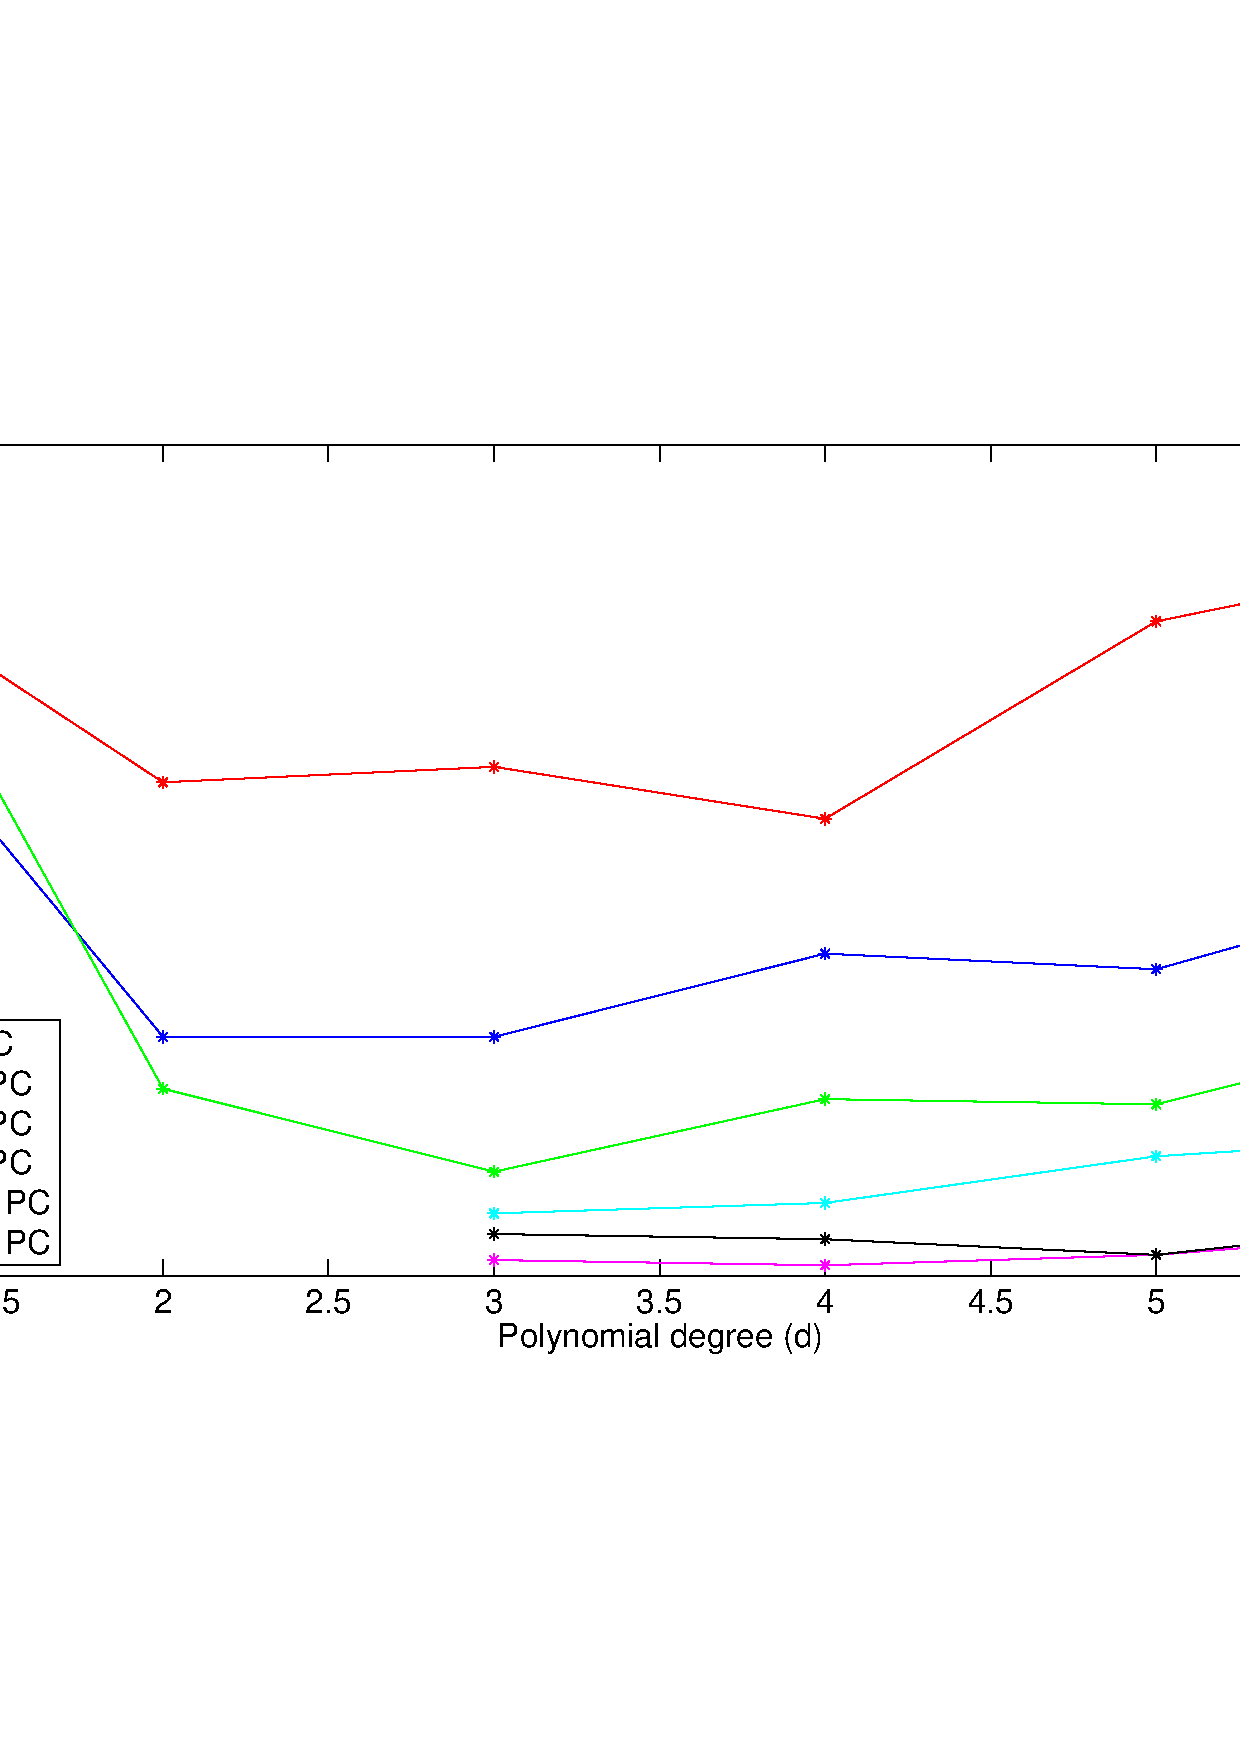
\includegraphics[width=\textwidth]{img/errorplotGMMclass.pdf}
    \caption{Classification errors using \texttt{classify} for different degrees of polynomial kernel and different numbers of principal components. The classification for a number of principal components higher than the dimension of the observations was only possible for polynomial degree $d>2$.}
    \label{fig:GMM}
\end{figure}

However, in the article \citep{scholkopf1997kernel} they used a linear Support Vector Machine (SVM) classifier and not just any linear classifier. The results using linear SVM can be seen in Figure \ref{fig:SVM}. Here we see that the best classification performance for linear PCA, $d=1$, was reached for 512 principal components and that was 6.6\%. The worst performance for $d=1$ was with 64 principal components with an error of 7.3\%. We notice that even the worst performance is better than the best performance we found for the previous classifier. If we then consider higher polynomial degrees $d>1$, we notice that the best performance for all numbers of principal components is achieved at polynomial degree 3 or 4 depending on the number of principal components extracted and for degrees higher than that the error increases again. Overall the level of error corresponds well with the original article's results but we do not get the same pattern in the results as we got for the previous classifier.
Also, since we do not know which type of multiclass SVM was used, one-vs-all or one-vs-one, whether a slack was used or not and how large and how compliant was the slack, we could not reproduce the exact results described in the paper.

\begin{figure}
    \centering
    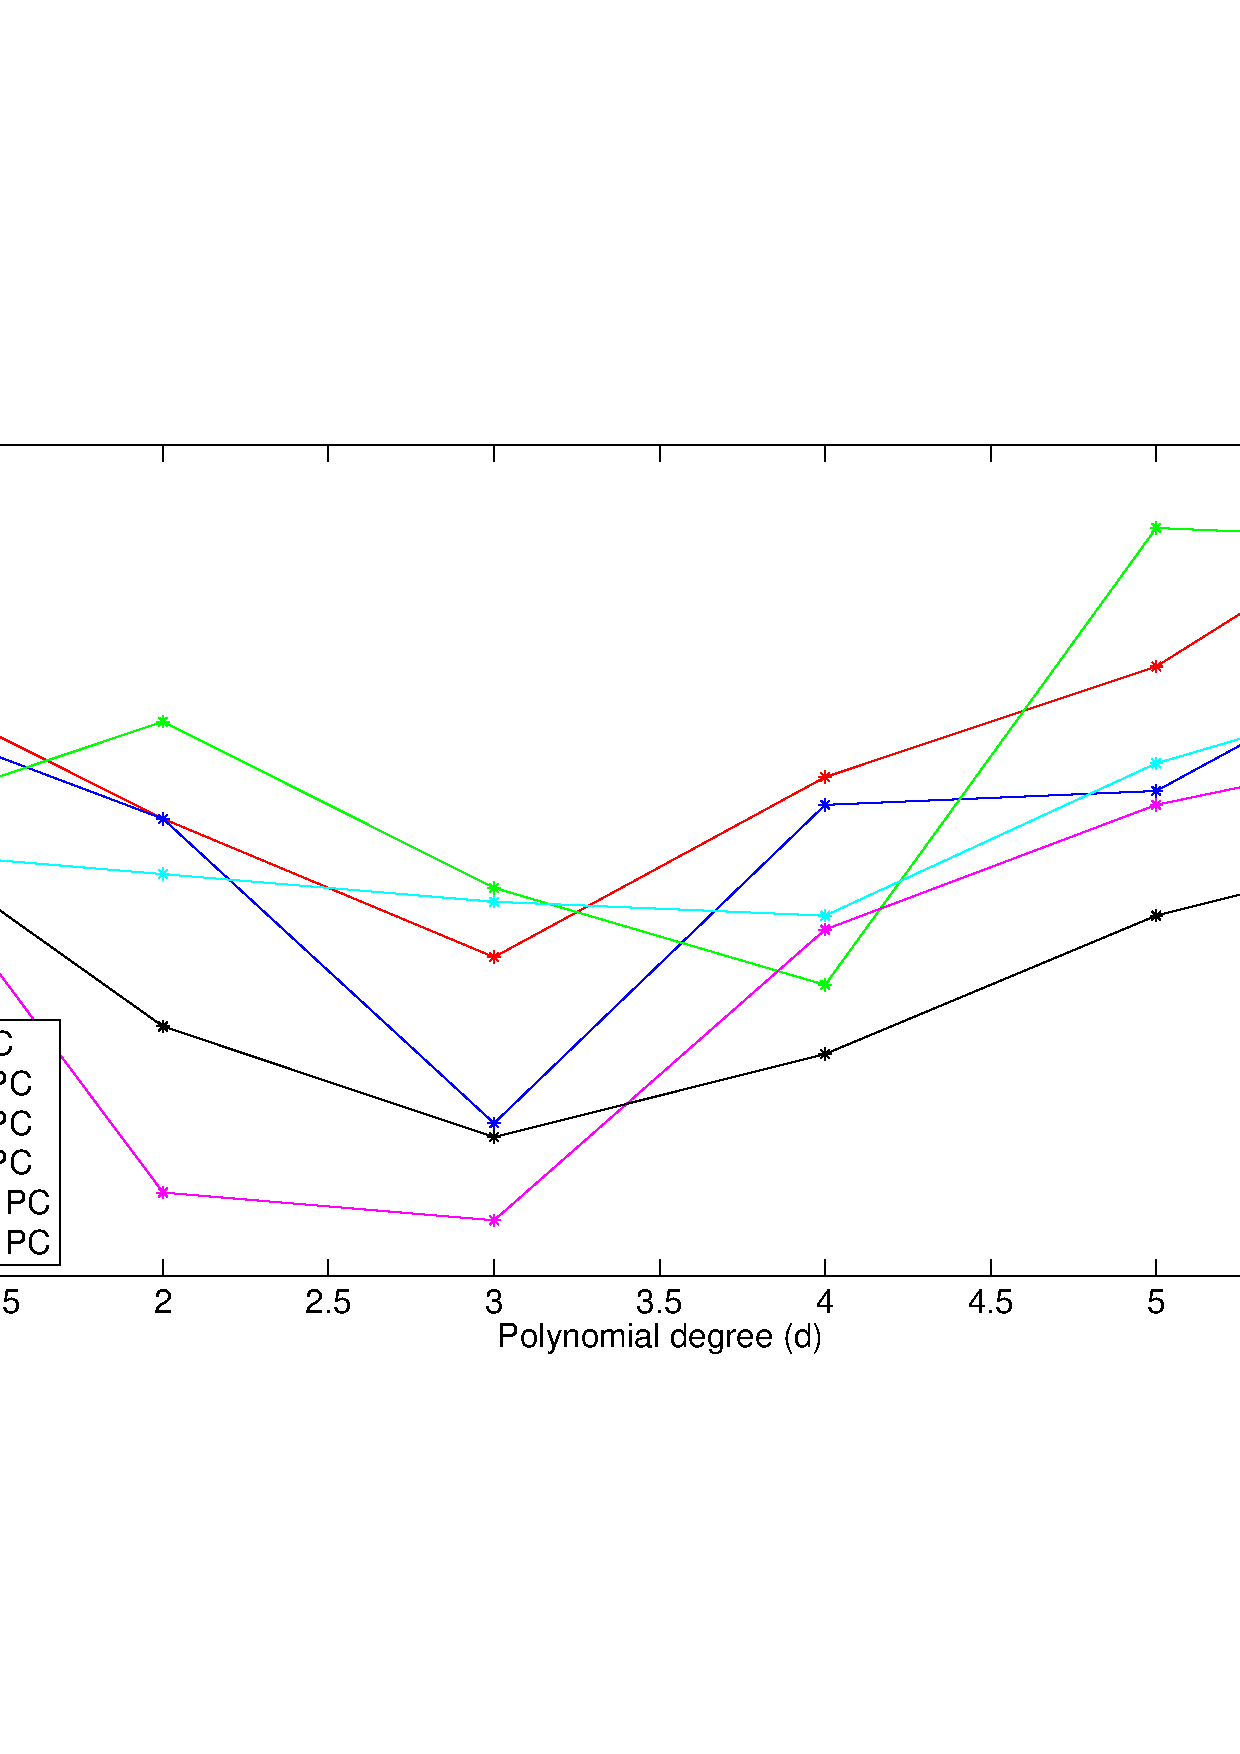
\includegraphics[width=\textwidth]{img/errorplotSVMclass.pdf}
    \caption{Classification errors using linear SVM classifier for different degrees of polynomial kernel and different numbers of principal components.}
    \label{fig:SVM}
\end{figure}


Generally, we were able to recreate their experiment even though all our error rates do not correspond exactly to the ones obtained in the original article. This can be due to differences in the linear classifiers because of different parameters or simply improvements in the implementations of these classifiers since the article was published in 1997.
    \section{Discussion}
Kernel PCA proposes an efficient way to compute principal components on a high-dimensional feature space that is related to the input space in a non-linear way. It does that by using a kernel to represent the dot product between two vectors in the feature space. This means that it can better describe non-linearities in the data.
In our experiments non-linear Kernel PCA gave better results than standard linear PCA when extracting features and classifying using a linear classifier. This is advantage that could replicate from the original article. 
Another advantage is that we only need to solve an eigenvalue problem, as we do in standard PCA, and not use any non-linear optimization method. This is an advantage over other forms of non-linear PCA \cite{scholkopf1997kernel}.

The paper introduces several different kernels that can be used in the method and have previously been successfully used in Support Vector Machines. This knowledge can be used in kernel PCA but also in any other algorithm that only requires the inner product between vectors. However, the article only describes results from experiments for a polynomial kernel function. It would be interesting to reproduce the experiment using a different kernel function, and see how well this algorithm performs. In general use a kernel that is specific to the problem in order obtain a better performance.

The kernel PCA is not suitable for large datasets as PCA is not, since the method is computationally expensive and we cannot fit our data using conventional data structures in RAM and an out-of-core computation is required \cite{halko2011algorithm}. It would be interesting to adapt current PCA algorithms that attempt to take care of these computational problem to a kernel PCA method.

Eventually, we have noticed that when we computed the covariance matrix, $\bar{C}$, in derivation of the method, then the scaling factor applied was $l$. Since the use of this factor would induce a bias \cite{farebrother1999fitting}, we propose to improve the Kernel PCA method by using the Bessel's correction and therefore using $l - 1$ as a scaling factor to remove the bias. This is relevant because the method exclusively rely on the variance. This would change the eigenvalue problem slightly and thereby the normalization of the eigenvectors.

    \pagebreak
    
    \bibliographystyle{plain}
    \renewcommand{\bibname}{References}
    \bibliography{references}

    %\backmatter
\end{document}
